\section{Methods}
% briefly explain the processes
% mention which parameters that are affected by size
%
\subsection{Model description}
The model and its four state variables are illustrated in Figure \cref{fig:ModelIllust}. For each state variables, the given biological and physical processes has been divided into gains or losses.  
\begin{figure}[H]
\centering
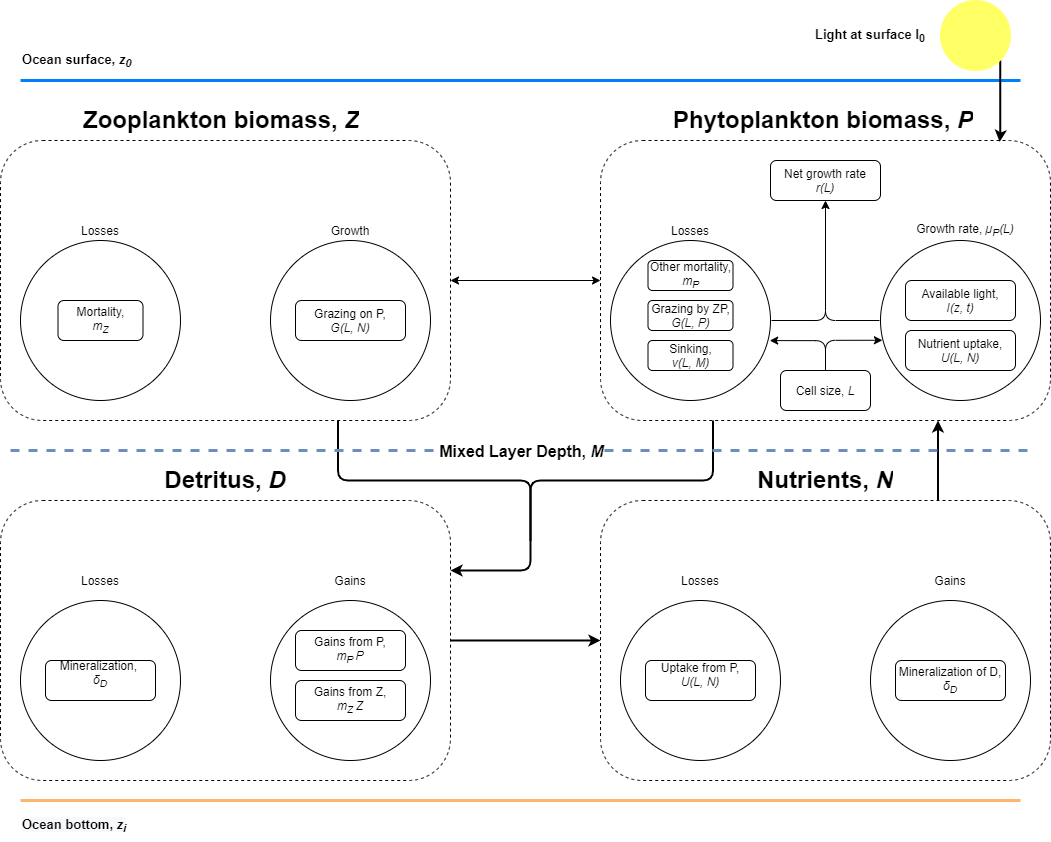
\includegraphics[width=.90\linewidth]{Figures/ModelIllustration_HighRes1.png}
\caption{The model illustration is highlighting the gains and losses for each of the state variables. Processes described in boxes marked by red is dependent on the mean cell size L.}
\label{fig:ModelIllust}
\end{figure}
Phytoplankton is either grazed upon by zooplankton or turned into detritus when dying. Similarly, zooplankton are turned into detritus, which sink while being remineralized into dissolved inorganic nutrients. The cycle is then closed as the phytoplankton take up nutrients and light, which is converted into growth. 
\newline
\newline
In our trait-based model, the cell size of phytoplankton is the mean trait described with a log-normal size distribution: $\mathrm{L=log(S)}$. S is the Equivalent Spherical Diameter (ESD) given in \si{\mu m}. The change in mean cell size over time is described by the following equation
\begin{equation}
    \label{eq:changecellsize}
    \mathrm{\frac{d\bar{L}}{dt} = V\frac{\partial r(\bar{L})}{\partial L}},
\end{equation}
where r is the net growth rate of phytoplankton, which is given in Equation \eqref{eq:netgrowthrateP}. V is the variance of the log size diversity of the phytoplankton community, which represents a way of measuring functional diversity. In contrast to \cite{AcevedoTrejos2015} who modelled the variance as $\mathrm{\frac{dV}{dt}=-V^2\frac{\partial^2 r(\bar{L}) }{\partial^2 L}+\delta_I(V_0-V)}$, we defined the variance as a constant of 0.16 \si{[Log\mu m \ ESD]^2}, to make to simplify the model. This value was chosen based on the mean size variance for tropical regions found by \cite{AcevedoTrejos2015}, which showed very small fluctuations for these systems.
%KEN: Jeg har lavet en skitse der viser fordelingerne af størrelserne. I virkeligheden er der jo en fordeling af cellestørrelser, p(L), som har en spredning, sigma. Variancen er proportional med sigma^2. I artiklen modellerer de både hvordan variancen og middelværdien ændrer sig. Vi må lave en antagelse omkring variancen.
%Det ville være logisk at beskrive V med en “coefficient of variation”, dvs antage at V er proportional til L^2 (V har jo enheden L^2). På den måde bliver V mindre når L bliver mindre, og så bliver dL/dt også mindr
\newline
\newline
M(t) is a forcing function describing how the mixed layer depth (MLD) changes with seasons. As the MLD is relatively constant in the tropical region modelled by \cite{AcevedoTrejos2015}, we decided to set it equal to XXX m instead. This implies that the change of the mixed layer depth, h(t), is assumed to be zero over an entire year, independently of seasonality. Hence, our model does not take into account any effects of entrainment and detrainment, as they do in \cite{AcevedoTrejos2015}.
\newline
\newline
%Entrainment and detrainment are taken into account in the term $\mathrm{h^{+} = max[h(t),0]}$. 
The diffusive mixing K is then given by the following equation:
\begin{equation}
    \label{eq:K}
    \mathrm{K = \frac{\kappa}{M}},
\end{equation}
where $\kappa$ is the cross-thermocline mixing. 
%The actual change $\mathrm{h(t)}$ in the MLD per day is defined as,
%\begin{equation}
 %   \label{eq:h(t)}
  %  \mathrm{h(t) = \frac{dM(t)}{dt}}
%\end{equation}


\subsection{System of equations}
The changes in the total biomass of the phytoplankton (P) community over time is given as a function of cell size:
\begin{equation}
    \label{eq:phytoplanktonbiomass}
    \mathrm{\frac{dP}{dt} = r(\bar{L})P}
\end{equation}
The net growth rate of P, $\mathrm{r(\bar{L}})$, can be written as
\begin{equation}
    \label{eq:netgrowthrateP}
    \mathrm{r(\bar{L})=\mu_{Pmax}f(T)\Psi(I)U(\bar{L},N)+\delta_I-m_P-\mu_ZG(\bar{L},P)Z-v(\bar{L},M)-K},
\end{equation}
where $\mathrm{\delta_I}$ is the rate of dispersal of phytoplankton from patches nearby into the community of interest, K is the mixing, $\mathrm{G(L,P)}$ is the zooplankton grazing, $\mathrm{v(L,M)}$ is the phytoplankton sinking and $\mathrm{m_P}$ represents any other losses of P. \textit{Explain the terms in the first part of equation. Mention that PAR = constant.}
\newline
\newline
\textbf{Nutrient uptake of phytoplankton}
\newline
%The growth rate of phytoplankton $\mathrm{\mu_P(N,I)}$ is limited by two factors, which are the light and the available nutrients. The least abundant is controlling the growth, which is in accordance with Liebig's law of the minimum:
%\begin{equation}
  %  \label{eq:growthrate}
   % \mathrm{\mu_P(N,I) = %\mu_{Pmax}f(T)\Psi(I)U(\bar{L},N)},
%\end{equation}
%where $\mathrm{\mu_{Pmax}}$ is maximum specific growth rate of P, I is the light intensity and $\mathrm{H_{I}}$ is the half saturation constants of light limited growth. 
U is the phytoplankton nutrient uptake as a function of nutrients N and the cell size of phytoplankton L, given by
\begin{equation}
    \label{eq:nutrientuptake}
    \mathrm{U(L,N) = \frac{N}{H_N+N}=\frac{N}{(\beta_U\cdot e^{L\alpha_U})+N}},
\end{equation}
where $\mathrm{\beta_U}$ is the intercept of the allometric function $\mathrm{H_N}$ (the half-saturation for nutrients) and $\mathrm{\alpha_U}$ is the slope of $\mathrm{H_N}$.
% we need to discuss the consequence of this somewhere
%\newline
%The light intensity is given in accordance with Lambert–Beer’s law, which means that it is decreasing exponentially with depth as a result of light being absorbed by biomass, water and other substances:
%\begin{equation}
 %   \label{eq:light}
 %   \mathrm{I(z,t) = I_{in}exp \bigg( - \int_{0}^{z} k_{p}P(\sigma,t) \,d \sigma - K_{bg}z \bigg)},
%\end{equation}
%where $\mathrm{I_{in}}$ is the incident light intensity, $\mathrm{k_p}$ is the phytoplankton light absorption coefficient, $\mathrm{K_{bg}}$ is the background turbidity of the water and $\mathrm{\sigma}$ is an integration variable. 
\newline
\newline
\textbf{Phytoplankton sinking}
\newline
Based on Stokes' law, the phytoplankton sinking $\mathrm{v(L,M)}$ is given as a function of cell size and the forcing function $\mathrm{M(t)}$.
\begin{equation}
    \label{eq:sinking}
    \mathrm{v(L,M) = \frac{\beta_v\cdot e^{L\cdot \alpha_v}}{M(t)}}
\end{equation}
The constants $\mathrm{\alpha_v}$ and $\mathrm{\beta_v}$ are the slope and the intercept of the allometric function v, respectively. This indicates that higher cells have higher sinking rates, meaning that they will be transported away from the mixed layer at a faster rate than smaller cells. 
\newline
\newline
\textbf{Zooplankton grazing}
\newline
The zooplankton grazing G(L,P) is also scaling with the cell size of phytoplankton, where the grazing pressure decreases with increasing cell size. It can be described by the Michaelis-Menten type function
\begin{equation}
    \label{eq:grazing}
    \mathrm{G(L,P) = \frac{e^{L\cdot\alpha_G}}{P\cdot e^{L\cdot \alpha_G}+H_P}},
\end{equation}
where $\mathrm{H_P}$ is the half saturation constant for grazing and $\mathrm{\alpha_G}$ is the slope for the allometric grazer preference.
\newline
\newline
\textbf{Model dynamics}
\newline
The final differential equations describing nutrients (N), phytoplankton (P), zooplankton (Z), and detritus (D) are then given by
% nutrients
\begin{equation}
    \label{eq:Ndynamics}
    \mathrm{\frac{dN}{dt} = -\mu_P(N,I)P+\delta_D D+K(N_0-N)}
\end{equation}
% phytoplankton
\begin{equation}
    \label{eq:Pdynamics}
    \mathrm{\frac{dP}{dt} = \left[ \mu_P(N,I)+\delta_I-m_P-\mu_ZG(\bar{L},P)Z-v(\bar{L},M)-K \right] P}
\end{equation}
% zooplankton
\begin{equation}
    \label{eq:Zdynamics}
    \mathrm{\frac{dZ}{dt} = \delta_Z\mu_Z G(\bar{L},P)PZ-m_Z Z^2 - \frac{h(t)}{M(t)}Z}
\end{equation}
%detritus
\begin{equation}
    \label{eq:Ddynamics}
    \mathrm{\frac{dD}{dt} = (1-\delta_Z)\mu_Z G(\bar{L},P)PZ+m_P+m_Z Z^2-\delta_D D-KD}
\end{equation}
%
\subsection{Parameters}
A table showing all the parameters used in the model...

\begin{table}[H]
\centering
\caption{Parameters and variables used for the model simulations.}
\label{tab:paramvariables}
\begin{tabular}{
>{\columncolor[HTML]{EFEFEF}}l 
>{\columncolor[HTML]{EFEFEF}}l 
>{\columncolor[HTML]{EFEFEF}}l 
>{\columncolor[HTML]{EFEFEF}}l }
\hline
Symbol & Meaning                                             & Value & Units             \\ \hline
\multicolumn{4}{l}{\cellcolor[HTML]{EFEFEF}\textit{Independent variables}}               \\
t      & Time                                                &       & d                 \\
$\bar{L}$      & Mean phytoplankton cell size                                                &       & \si{\mu m}                 \\
\multicolumn{4}{l}{\cellcolor[HTML]{EFEFEF}\textit{Dependent variables}}  \\ 

N      & Nutrients          &  -    &  mmol N \si{m^{-3}}  \\
P                    & Pythoplankton biomass                        & -      &  mmol N \si{m^{-3}}  \\
Z                        & Zooplankton biomass                       & -      &  mmol N \si{m^{-3}} \\
D                            & Detritus biomass                       & -     &  mmol N \si{m^{-3}}  \\
\multicolumn{4}{l}{\cellcolor[HTML]{EFEFEF}\textit{Parameters}}                          %\\ $I_{in}$    & Incident light intensity                            & 300    & \si{\mu mol} photons \si{m^{-2}} \si{s^{-1}} 
%\\ $K_{bg}$    & Background turbidity of water                       & 0.045 & \si{m^{-1}}  
\\ M & Mixed layer depth (MLD)  & 10-100     &  m  \\ $\mathrm{N_0}$ & Nutrient concentration below the MLD  & 2-50     &  mmol N \si{m^{-3}} \\
$\mathrm{\Psi}$ & Photosynthetically active radiation                    & 40     &  \si{Ein} \si{m^{-2}} \si{d^{-1}}  \\ T & Temperature  & 25     &  \degree C  \\ $\mathrm{\kappa}$                    &
Cross thermocline mixing                    &  0.01   &  m \si{d^{-1}}   \\ $\mathrm{K_P}$ & P half saturation  & 0.1     &  mmol N \si{m^{-3}} \si{\mu m^{-1}} \\ $\mathrm{\delta_I}$ &  P immigration rate      & 0.008   &   \si{d^{-1}} \\
$\mathrm{m_p}$   & P mortality rate                & 0.05   & \si{d^{-1}}  \\
$\mathrm{\mu_{Pmax}}$        &        P max growth rate           & 1.4    & \si{d^{-1}}  \\
$\mathrm{\mu_Z}$  & Z growth rate                   & 1.1     & \si{d^{-1}} \\ $\mathrm{m_Z}$                    &
Z mortality rate     &  0.3   &  \si{d^{-1}}  \\  $\mathrm{\delta_D}$               & Mineralization rate                         &  0.1  &  \si{d^{-1}}   \\ $\mathrm{\delta_Z}$  
 & P assimilation coefficient                  & 0.3   &  -  \\
 $\mathrm{\beta_U}$  &  Intercept of the $K_N$ allometric function       & 0.14257  &  \\  $\mathrm{\alpha_U}$                    &
Slope of the $\mathrm{K_N}$ allometric function      &  0.81   &   \\ $\mathrm{\beta_v}$        & Intercept of the $\mathrm{v}$ allometric function    &  0.01989 &  \\ $\mathrm{\alpha_G}$                    & 
Slope for allometric grazer preference      &  -0.75   &  \\ $\mathrm{\alpha_v}$                    &
Slope of the $v$ allometric function        &  1.17   &   \\
\hline
\end{tabular}
\end{table}